\renewcommand*\thechapter{}
\renewcommand*\thesection{\Alph{section}}
\chapter*{Appendix}
\chaptermark{Appendix}
\stepcounter{chapter}
\ifoot{Appendix}
\addcontentsline{toc}{chapter}{Appendix}

\section{Schematic of the Riemann Pump circuit}
\label{app:schematic}
\begin{figure}[ht]
	\centering
  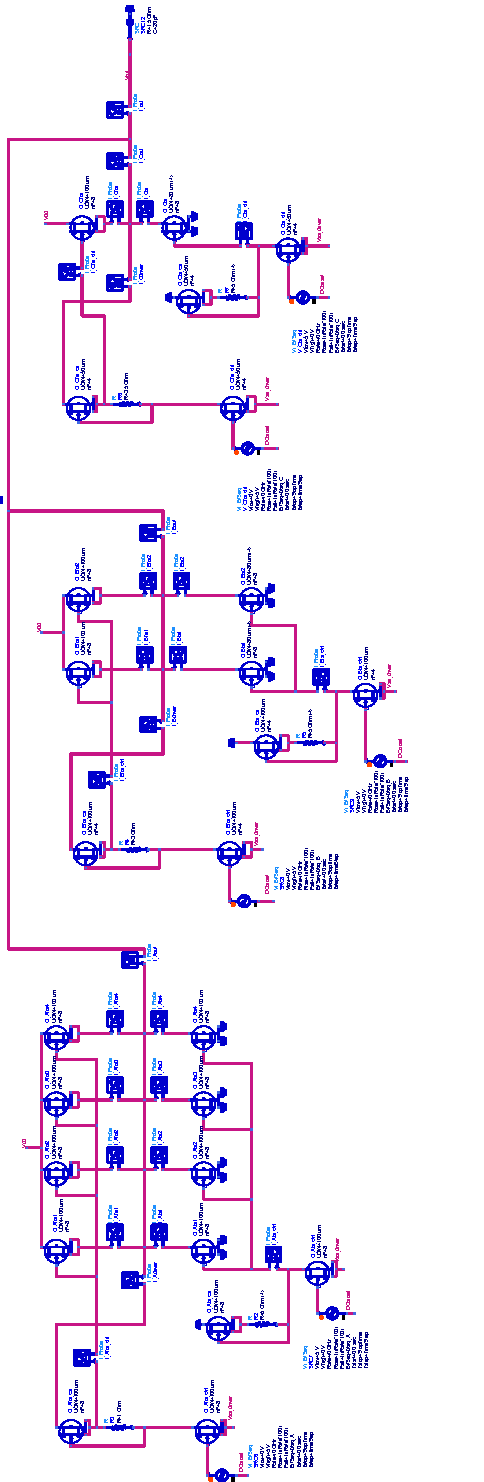
\includegraphics{CircuitSchematic_portrait.pdf}
	\caption{Realized circuit with \gls{ab:ads}}
	\label{fig:Circuitschematic}
\end{figure}

\newpage
\section{Layout of the whole Riemann Pump circuit}

bla bla bla bal bla lbal blalsl

bla bla bla bal bla lbal blalsl

\newpage
\section{Photography of the realized Demonstrator version 1}

\begin{figure}[htb!]
   \centering
   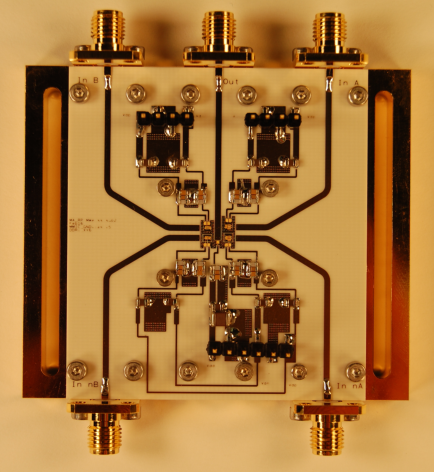
\includegraphics{Demonstrator.pdf}
   \caption{Photo demonstrator}
   \label{pic:DemonstratorDDRiXY6}
\end{figure}

\section{Photography of the realized Demonstrator version 2}

bla bla bla bal bla lbal blalsl